% !TEX encoding = UTF-8
\documentclass[UTF8]{ctexart}

\usepackage[utf8]{inputenc}
\usepackage{graphicx}
\usepackage{geometry}
\geometry{a4paper}
\geometry{left=2.5cm,right=2.5cm,top=2.8cm,bottom=1.3cm}

\usepackage{booktabs}
\usepackage{array}
\usepackage{paralist}
\usepackage{verbatim}
\usepackage{subfig}
\usepackage{amsmath}
\usepackage{mathtools}
\usepackage{listings}
\usepackage[table]{xcolor}
\usepackage{lastpage}
\usepackage{url}

% Using hyperref for improved ref character
\usepackage[colorlinks,linkcolor=black,anchorcolor=black,
citecolor=black,CJKbookmarks=True]{hyperref}

% For picture drawing
\usepackage[all]{xy}

% For code inserting. Set features.
\lstset{
alsolanguage=matlab,
tabsize=4,
keepspaces=true,
numbers=left,
numberstyle=\tiny,
keywordstyle=\color{blue!70} \bfseries,
commentstyle=\color{red!50!green!50!blue!50},
frame=shadowbox,
breaklines,
showspaces=false,
showstringspaces=false,
showtabs=false,
rulesepcolor=\color{red!20!green!20!blue!20},
extendedchars=false,
escapeinside=``
}

% Set the font of page header
\usepackage{fancyhdr}
\pagestyle{fancy}
\lhead{传感器特性实验报告}
\chead{}
\rhead{Page \thepage/\pageref{LastPage}}
\cfoot{}
\rfoot{}
\lfoot{}

\usepackage{sectsty}

\usepackage[nottoc]{tocbibind}
\usepackage[titles,subfigure]{tocloft}
\renewcommand{\cftsecfont}{\rmfamily\mdseries\upshape}
\renewcommand{\cftsecpagefont}{\rmfamily\mdseries\upshape}

% Set number of ref to be relevent to section number
\renewcommand{\theequation}{\arabic{section}.\arabic{equation}}
\renewcommand{\thefigure}{\arabic{section}-\arabic{figure}}
\renewcommand{\thetable}{\arabic{section}-\arabic{table}}
\makeatletter
\@addtoreset{equation}{section}
\@addtoreset{figure}{section}
\@addtoreset{table}{section}
\makeatother

% Set the font of the reference
\bibliographystyle{unsrt}

% Define user\rq{}s color
\usepackage{colortbl}
\definecolor{lightgray}{gray}{.9}
\definecolor{thickgray}{gray}{.6}

\usepackage{multirow}

% 首行缩进
\usepackage{indentfirst}

% Set section numbering
\CTEXsetup[number={}]{part}
\renewcommand{\thepart}{}
\usepackage{titlesec}
\titleformat{\part}[block]{\color{blue}\huge\bfseries\filcenter}{}{1em}{}

%\usepackage{ulem}
%\usepackage{indentfirst}
%\setlength\textwidth{300.0pt}
%

% 重定义字体命令
\newcommand{\song}{\CJKfamily{song}}    % 宋体   (Windows自带simsun.ttf)
\newcommand{\fs}{\CJKfamily{fs}}        % 仿宋体 (华天字库htfs.ttf)
\newcommand{\kai}{\CJKfamily{kai}}      % 楷体   (华天字库htkai.ttf)
\newcommand{\hei}{\CJKfamily{hei}}      % 黑体   (Windows自带simhei.ttf)
\newcommand{\li}{\CJKfamily{li}}        % 隶书   (Windows自带simli.ttf)
\newcommand{\you}{\CJKfamily{you}}      % 幼圆体 (Windows自带simyou.ttf)
%%%  以上六种字体均为标准 GBK 字体, 包括 GBK 繁体字和一些不常用字, 推荐!!!

\newcommand{\xs}{\CJKfamily{xs}}
\newcommand{\shu}{\CJKfamily{shu}}      % 舒体   (方正字库fzstk.ttf)
%  \newcommand{\yourcommand}[参数个数]{内容}   [参数个数]这个是可选的。
%  例如  \newcommand{\you}{\CJKfamily{you}}  用\you 来代替 \CJKfamily{you} ,少输入很多字哦。
%字号设置
\newcommand{\chuhao}{\fontsize{42pt}{\baselineskip}\selectfont}
\newcommand{\xiaochuhao}{\fontsize{36pt}{\baselineskip}\selectfont}
\newcommand{\yihao}{\fontsize{28pt}{\baselineskip}\selectfont}
\newcommand{\xiaoyihao}{\fontsize{24pt}{\baselineskip}\selectfont}
\newcommand{\erhao}{\fontsize{21pt}{\baselineskip}\selectfont}
\newcommand{\xiaoerhao}{\fontsize{18pt}{\baselineskip}\selectfont}
\newcommand{\sanhao}{\fontsize{15.75pt}{\baselineskip}\selectfont}
\newcommand{\sihao}{\fontsize{14pt}{\baselineskip}\selectfont}
\newcommand{\xiaosihao}{\fontsize{12pt}{\baselineskip}\selectfont}
\newcommand{\wuhao}{\fontsize{10.5pt}{\baselineskip}\selectfont}
\newcommand{\xiaowuhao}{\fontsize{9pt}{\baselineskip}\selectfont}
\newcommand{\liuhao}{\fontsize{7.875pt}{\baselineskip}\selectfont}
\newcommand{\qihao}{\fontsize{5.25pt}{\baselineskip}\selectfont}
% \baselineskip | distance from bottom of one line of a paragraph to bottom of the next line.  基本行距
%  只有使用\selectfont命令之后,\fontzize{}{}的设置才能生效
%  可以用数字表示{11pt}:单倍行距

\begin{document}
%%%%%%%%%%%%%%%%%%%%%%%%%%%%封面与目录%%%%%%%%%%%%%%%%%%%%%%%%%%%%%%
\begin{titlepage}
\begin{center}
% Upper part of the page

\includegraphics[width=0.25\textwidth]{resource/logo.jpg}\\[1cm]
\textsc{\LARGE Department of Automation}\\[1.5cm]
\fs{\Large 模式识别基础第四次作业}\\[0.5cm]
% Title
\hrulefill
\\[0.8cm]{\centering \huge \hei 用身高体重等数据进行聚类的实验}\\[0.4cm]
\hrulefill
\\[4cm]

% Author and supervisor
\begin{tabbing}       %tabbing  列表

 \hspace*{5cm} \= \hspace{2.6cm} \= \kill
 % \=     in tabbing environment, sets a tab stop
 % \kill  in a\tabbing environment, deletes previous line so tabs can be set without outputting text.
 % \>     in tabbing environment is a forward tab.

\>{\fs\sihao\textbf {班\hspace{1cm}级 \ \ :}}\>  {\centering\fs\sihao\textbf{~~~~~~~~~自~~3~2}} \\
\\
\>{\fs\sihao\textbf {姓\hspace{1cm}名 \ \ :}}\>  {\centering\fs\sihao\textbf{~~~~~~~~陈~昊~楠}}\\
\\
\>{\fs\sihao\textbf {学\hspace{1cm}号 \ \ :}}\>  {\centering\fs\sihao\textbf{~~~~~~2013011449}}\\
\\
\>{\fs\sihao\textbf {授课教师 \ \ :}}\>  {\centering\fs\sihao\textbf{~~~~~~~~张~学~工}} \\

\end{tabbing}
\vfill
{\large \today}
\end{center}
\end{titlepage}

\tableofcontents
\clearpage

%%%%%%%%%%%%%%%%%%%%%%%%%%正文部分%%%%%%%%%%%%%%%%%%%%%%%%%%%%%%%%%%

\section{实验内容}
\begin{enumerate}
\item 把数据{\ttfamily dataset3.txt} 作为未知样本集(即忽略每个样本的类别信息),用{\ttfamily PCA} 对{\ttfamily dataset3.txt} 进行降维,画出各个主成分上的方差,根据方差分布确定选取几个主成分来构成数据新的表示。
\item 在以上得到的主成分表示上,用$C$ 均值方法对全部样本进行聚类分析,试验$C=2,3,4,5,6 $几种情况,连同$C=1$ 的情况一起画出$C$ 个聚类的误差平方和随类别数变化的折线,观察能否用非监督学习方法发现样本中有意义的聚类。选择其中一个最可能有意义的$C^*$。将聚类结果以适当的方式显示出来,对聚类结果进行分析和讨论。
\item 分别用原始的十维特征和{\ttfamily PCA} 选出的主成分做分级聚类,考查采用不同特征、不同距离度量选项对结果的影响,讨论将数据聚为几类更合理。将聚类结果以适当的方式显示出来,对聚类结果进行分析和讨论。
\end{enumerate}

\section{方法概述}
\subsection{PCA降维}
该方法在上次实验中已经使用过。其基本思路是对所有原始特征进行线性组合(系数之和为1),使得变换之后样本特征的方差尽可能大,且得到的特征线性无关。详细原理不再赘述。

\subsection{K均值聚类}
也成为c均值聚类。该方法将样本分为K类,最小化每个类内样本与该类中心距离的和。即
\begin{equation}
\sum_{i=0}^{K}\min_{x_j\in C_i}(||x_j-\mu_i||)^2
\end{equation}
其中$\mu_i$为第$i$类所有样本的均值。由于该方法需要将各特征距离相加,为了使它们贡献相同,需要在聚类之前先进行归一化操作。

K均值聚类方法有以下不足之处:
\begin{enumerate}
\item 该方法假设每类样本所占的区域是凸的,且各向同性。如果样本的分布不满足这种假设,聚类效果将会变差。
\item 欧式距离不是一种归一化度量,在数据维数升高时,距离也会相应增大。在聚类之前先进行降维操作可以减小这种影响。
\end{enumerate}

\subsection{层次聚类}
层次聚类算法先将每个样本当做单独的类,之后根据某种类间相似性度量方法,将距离最小的两类合并为一类。不断迭代该步骤,最少可将样本聚为一类,并在其过程中聚合为任意数目的类别。与K均值聚类不同,层次聚类方法如果确定好了相似性度量方法,聚类结果是确定的,因此不需要重复多次。

常用的类间的相似性度量(也称作连接)方法有以下四种:
\begin{enumerate}
\item 最近距离:$\Delta(\Gamma_i,\Gamma_j)=\min_{y\in \Gamma_i, \tilde{y}\in \Gamma_j}\delta(y,\tilde{y})$;
\item 最远距离:$\Delta(\Gamma_i,\Gamma_j)=\max_{y\in \Gamma_i, \tilde{y}\in \Gamma_j}\delta(y,\tilde{y})$;
\item 均值距离:$\Delta(\Gamma_i,\Gamma_j)=\delta(m_i,m_j)$,$m_i,m_j$分别为两类的均值向量;
\item {\ttfamily Ward} 距离:$\Delta(\Gamma_i,\Gamma_j)=\sum_{y\in \Gamma_i}\sum_{\tilde{y}\in \Gamma_j}euclidean(y,\tilde{y})$。
\end{enumerate}
上式中$\delta$为某种样本间的距离函数,如欧氏距离。以上四种方法中,最近距离和最远距离可以通过更换样本间距离度量而互换,实验中仅采用了最远距离。另外,最近、最远距离存在强者更强的问题,即在某一类本身就有很多样本时,往往更容易找到另一个最近或最远距离较小的类与之合并。{\ttfamily Ward} 距离可以很好解决这个问题,因为某类存在过多样本时,与其他类的总距离会变得很大,而难以继续扩展。均值距离也可以一定程度解决这个问题,因为当某类存在很多样本时,样本中心会远离该类的外沿,与其他类的距离会相应较大。并且均值距离可以选择各种样本距离度量方式,比{\ttfamily Ward} 距离更灵活。

\subsection{轮廓系数}
轮廓系数可以评价聚类的效果。对于某个样本$x_j$,用$a_j$表示该样本与同类的其他样本之间的平均距离,用$b_j$表示该样本与除该类之外其他各类所有样本平均距离的最小值。则样本点$x_j$的轮廓系数值为,
\begin{equation}
s_j=\frac{b_j-a_j}{\max\{a_j, b_j\}}.
\end{equation}

根据定义有$-1<s_j<1$。当$b_j\gg a_j$,$s_j$接近$1$,这时样本$x_j$的归类比较合适。整个数据集的轮廓系数定义为所有样本轮廓系数的均值。该值越接近$1$聚类效果越好。

\subsection{t-SNE降维}
t-distributed stochastic neighbor embedding ({\ttfamily t-SNE}) 是一种非线性降维的方法,非常适合将高维数据转化为2、3维并用于显示。该方法能很好保持在高维的间距,效果通常优于{\ttfamily PCA} 等线性降维方法。详细原理参见维基百科 \url{https://en.wikipedia.org/wiki/T-distributed_stochastic_neighbor_embedding}。

\section{实验结果}
\subsection{PCA降维}
使用{\ttfamily PCA}降维,各主成分方差和累计方差如图\ref{fig:pca}。由图可见,前4个主成分保留了$50\%$以上的方差,因此在下面的实验中均使用前4个主成分作为特征。

\begin{figure}
\centering
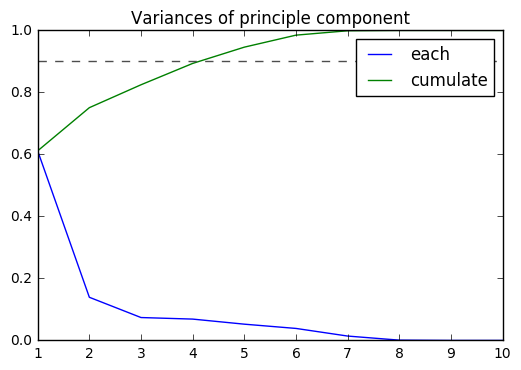
\includegraphics[width=11cm]{resource/pca.png}
\caption{{\ttfamily PCA}各主成分方差和累计方差}
\label{fig:pca}
\end{figure}

\subsection{K均值聚类}
\paragraph{聚类效果评价} 使用不同的类别数得到的聚类结果如表\ref{tab:kmeans},每个类别数的实验均执行10次。聚类误差平方和与类别数的关系如图\ref{fig:class}。由图线看不出明显的拐点,在K均值方法下,很难找出有明显意义的分类。从轮廓系数也可以看出,各种类别数下的轮廓系数比较接近,说明聚类没有明显的优劣。

\begin{table}[htbp]
\centering
\begin{tabular}{cccc}
\toprule
{} &   time &  inertia & silhouette \\
\midrule
class=2 &  0.11s &  3104.63 &      0.210 \\
class=3 &  0.09s &  2682.34 &      0.185 \\
class=4 &  0.10s &  2276.04 &      0.188 \\
class=5 &  0.09s &  1985.37 &      0.197 \\
class=6 &  0.11s &  1790.47 &      0.192 \\
class=7 &  0.12s &  1642.08 &      0.199 \\
class=8 &  0.15s &  1529.98 &      0.212 \\
class=9 &  0.16s &  1426.02 &      0.183 \\
\bottomrule
\end{tabular}
\caption{(10次实验)K均值聚类用时、聚类误差平方和与轮廓系数}
\label{tab:kmeans}
\end{table}

\begin{figure}
\centering
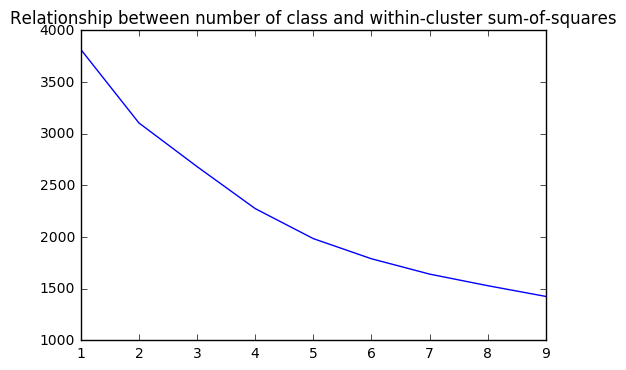
\includegraphics[width=11cm]{resource/class.png}
\caption{{\ttfamily PCA}各主成分方差和累计方差}
\label{fig:class}
\end{figure}

\paragraph{聚类结果显示} 使用{\ttfamily t-SNE} 算法将高维数据降至二维,不同类别的聚类结果如图\ref{fig:kmeans}。

\begin{figure}
\centering
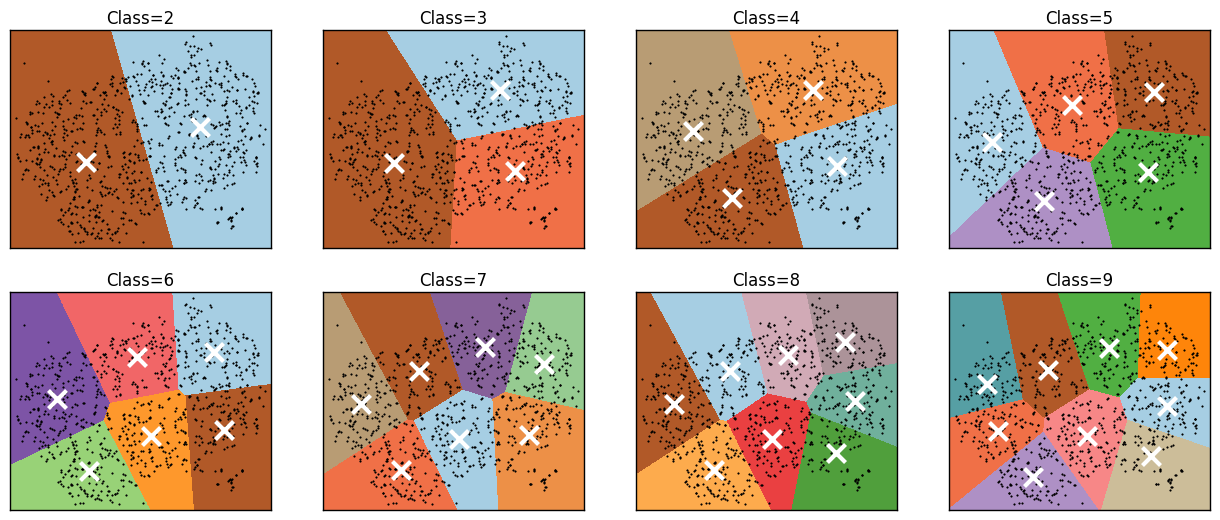
\includegraphics[width=15cm]{resource/k_means.png}
\caption{不同类别数的聚类结果}
\label{fig:kmeans}
\end{figure}

\subsection{层次聚类}
\paragraph{聚类效果评价} 层次聚类实验结果如表\ref{tab:hierarchical}。由表可见,当使用原始数据,使用均值距离代表类间距,且分为两类时,轮廓系数最大,聚类效果最好。这个结论和上一次作业中发现的{\ttfamily PCA} 降维后分类准确率降低比较吻合。这说明降维之后信息有损失,无论监督的分类还是无监督的聚类,效果都会变差。

\begin{table}[htbp]
\centering
\begin{tabular}{cccc}
\toprule
{} &    ward & average & complete \\
\midrule
orig, class=2 &  0.3416 &  \textbf{0.7155} &   0.5554 \\
orig, class=3 &  0.2383 &  0.4675 &   0.2718 \\
orig, class=4 &  0.1455 &  0.2589 &   0.1671 \\
orig, class=5 &  0.1401 &  0.2215 &   0.1632 \\
orig, class=6 &  0.1208 &  0.1654 &   0.1527 \\
orig, class=7 &  0.1156 &  0.2698 &   0.1478 \\
orig, class=8 &  0.1183 &  0.2374 &   0.1476 \\
orig, class=9 &  0.1073 &  0.1587 &   0.0970 \\
dcp4, class=2 &  0.1511 &  0.6773 &   0.3526 \\
dcp4, class=3 &  0.1154 &  0.5860 &   0.3512 \\
dcp4, class=4 &  0.1380 &  0.4304 &   0.3354 \\
dcp4, class=5 &  0.1599 &  0.3527 &   0.1525 \\
dcp4, class=6 &  0.1526 &  0.2983 &   0.1475 \\
dcp4, class=7 &  0.1524 &  0.2646 &   0.1375 \\
dcp4, class=8 &  0.1565 &  0.2562 &   0.1305 \\
dcp4, class=9 &  0.1434 &  0.2373 &   0.1265 \\
dcp2, class=2 &  0.3449 &  0.5382 &   0.5382 \\
dcp2, class=3 &  0.3316 &  0.4925 &   0.3040 \\
dcp2, class=4 &  0.3492 &  0.4171 &   0.3233 \\
dcp2, class=5 &  0.3314 &  0.3162 &   0.3494 \\
dcp2, class=6 &  0.2934 &  0.3067 &   0.3472 \\
dcp2, class=7 &  0.2834 &  0.3159 &   0.2920 \\
dcp2, class=8 &  0.2770 &  0.3134 &   0.2760 \\
dcp2, class=9 &  0.2858 &  0.2842 &   0.2950 \\
\bottomrule
\end{tabular}
\caption{层次聚类不同预处理方式、相似性度量、分类数下的轮廓系数。其中{\ttfamily orig} 表示原始数据,{\ttfamily dcp4} 表示经{\ttfamily PCA} 压缩至4维的数据,{\ttfamily dcp2} 表示经{\ttfamily PCA} 压缩至2维的数据。{\ttfamily ward}表示{\ttfamily Ward} 距离,,{\ttfamily average}表示均值距离{\ttfamily complete}表示最大距离。}
\label{tab:hierarchical}
\end{table}

\paragraph{聚类结果显示} 使用{\ttfamily Ward} 距离、最大距离、均值距离的分类结果分别如图\ref{fig:ward},图\ref{fig:complete}和图\ref{fig:average}。由图可见,{\ttfamily Ward} 距离确实能够得到样本数目比较相当的分类,均值、最大距离均存在类别的样本数不均衡的问题,分类数较大时更为明显。

\begin{figure}
\centering
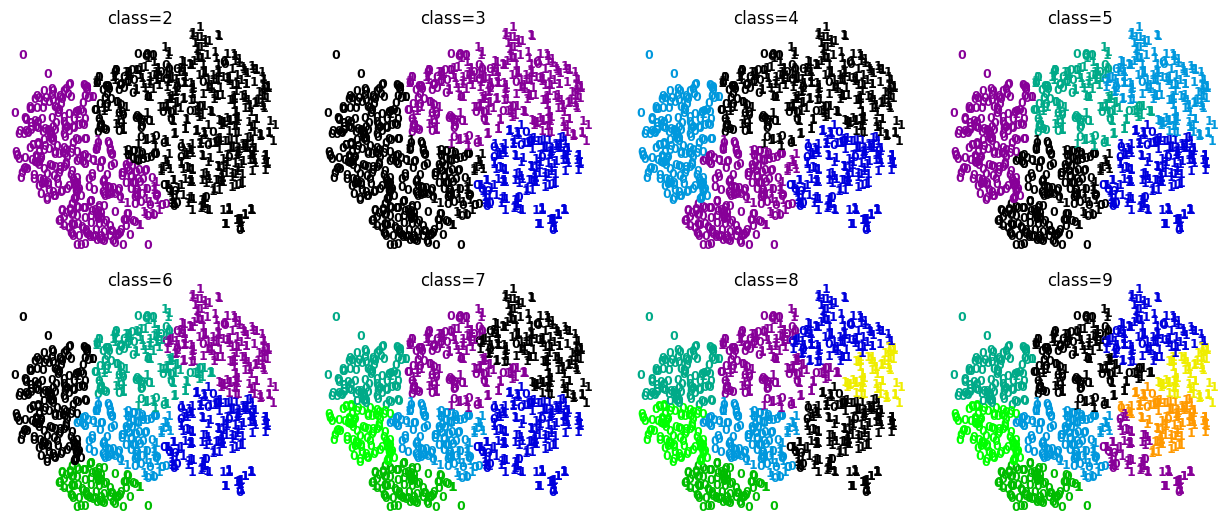
\includegraphics[width=15cm]{resource/ward.png}
\caption{{\ttfamily Ward} 距离层次聚类结果}
\label{fig:ward}
\end{figure}

\begin{figure}
\centering
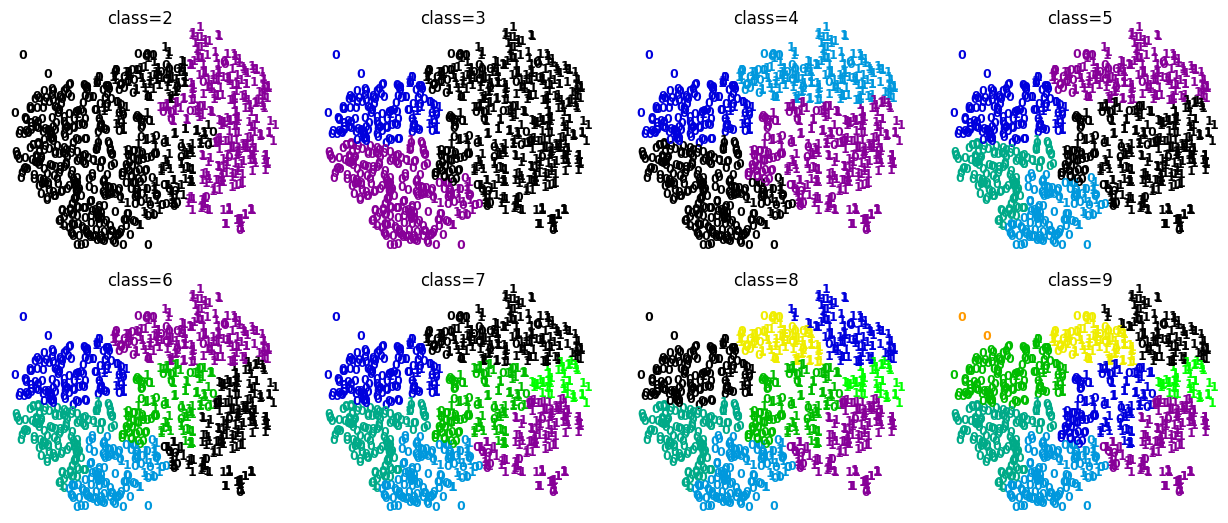
\includegraphics[width=15cm]{resource/complete.png}
\caption{最大距离层次聚类结果}
\label{fig:complete}
\end{figure}

\begin{figure}
\centering
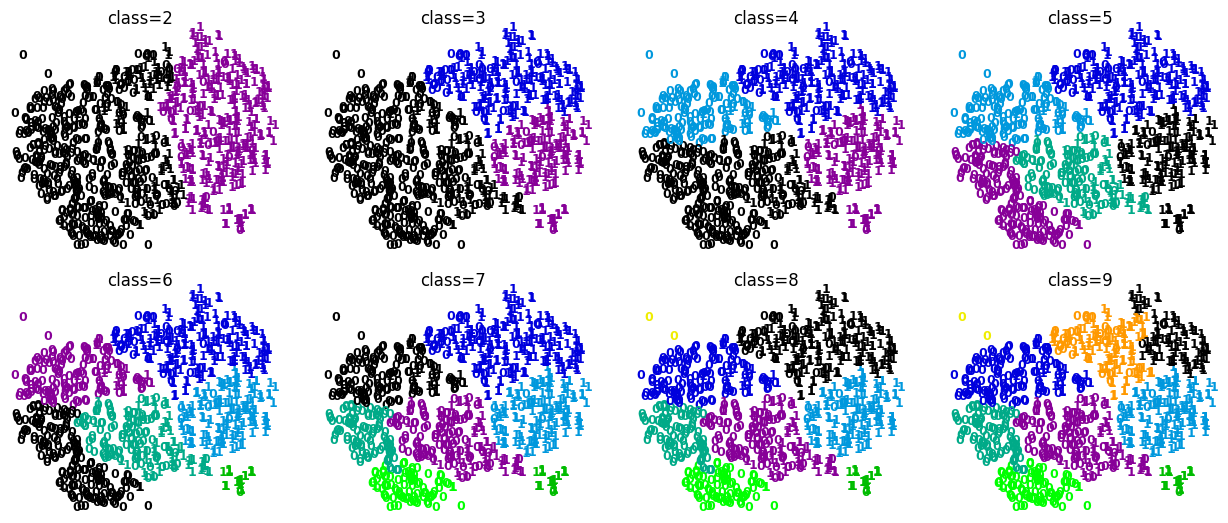
\includegraphics[width=15cm]{resource/average.png}
\caption{均值距离层次聚类结果}
\label{fig:average}
\end{figure}

\subsection{聚类分类准确率}
聚类数目为2时模型可能能够学习到性别的分类。为了验证这种猜想,实验中比较了各种方法在聚类数为2时与真实性别标签的偏差。结果如表\ref{tab:class}(其中K均值聚类为10次实验的平均结果)。由表可见,仅在不进行PCA降维时,使用{\ttfamily Kmeans} 聚类和{\ttfamily Ward} 度量的层次聚类能够与性别标签恰好有关。进一步,表\ref{tab:prop}显示了聚类之后样本数较多的一类在所有样本中所占的比重。由表可见,使用最大距离和平均距离度量的层次聚类方法均产生了严重的偏差。

应当说明的是,聚类得到的结果和性别分类没有必然关系。不过这种关系一定程度上反映了该数据集在性别标签下的可分性。另外需要说明的是,表\ref{tab:prop}所示的结果是经过{\ttfamily PCA}降维的,而图\ref{fig:complete}、图\ref{fig:average}所示的结果是经过{\ttfamily t-SNE} 降维的,这是一种非线性降维方法,对于最大距离和均值分类没有显示出明显的偏差。作为补充,图\ref{fig:pca_dec}给出了使用{\ttfamily PCA} 降维的均值距离层次聚类结果。可以看出,这个结果明显有偏差,是因为{\ttfamily PCA} 对一些特殊样本的处理不好,个别样本和其他样本的距离差距过大。

\begin{table}[htbp]
\centering
\begin{tabular}{cccccc}
\toprule
{} &   pca=2 &   pca=4 &   pca=6 &   pca=8 &  pca=No \\
\midrule
Kmeans, km++ init   &  0.5419 &  0.5335 &  0.5419 &  0.5356 &  \textbf{0.8952} \\
Kmeans, random init &  0.5419 &  0.5419 &  0.5356 &  0.5335 &  \textbf{0.8952} \\
Hier, ward          &  0.5566 &  0.5566 &  0.5566 &  0.5566 &  \textbf{0.9036} \\
Hier, average       &  0.5073 &  0.5073 &  0.5073 &  0.5073 &  0.5073 \\
Hier, complete      &  0.5199 &  0.5199 &  0.5199 &  0.5199 &  0.5021 \\
\bottomrule
\end{tabular}
\caption{聚类与性别标签的相关性,分类准确率结果。其中pca=x意为使用PCA将数据降到x维,pca=No表示不对数据进行降维。}
\label{tab:class}
\end{table}

\begin{table}[htbp]
\centering
\begin{tabular}{cccccc}
\toprule
{} &   pca=2 &   pca=4 &   pca=6 &   pca=8 &  pca=No \\
\midrule
Kmeans, km++ init   &  0.5136 &  0.5157 &  0.5115 &  0.5115 &  0.5294 \\
Kmeans, random init &  0.5136 &  0.5136 &  0.5136 &  0.5105 &  0.5294 \\
Hier, ward          &  0.6017 &  0.6017 &  0.6017 &  0.6017 &  0.5000 \\
Hier, average       &  0.9990 &  0.9990 &  0.9990 &  0.9990 &  0.9990 \\
Hier, complete      &  0.9549 &  0.9549 &  0.9549 &  0.9549 &  0.9937 \\
\bottomrule
\end{tabular}
\caption{不同聚类方法大类所占比例。其中pca=x意为使用PCA将数据降到x维,pca=No表示不对数据进行降维。}
\label{tab:prop}
\end{table}

\begin{figure}
\centering
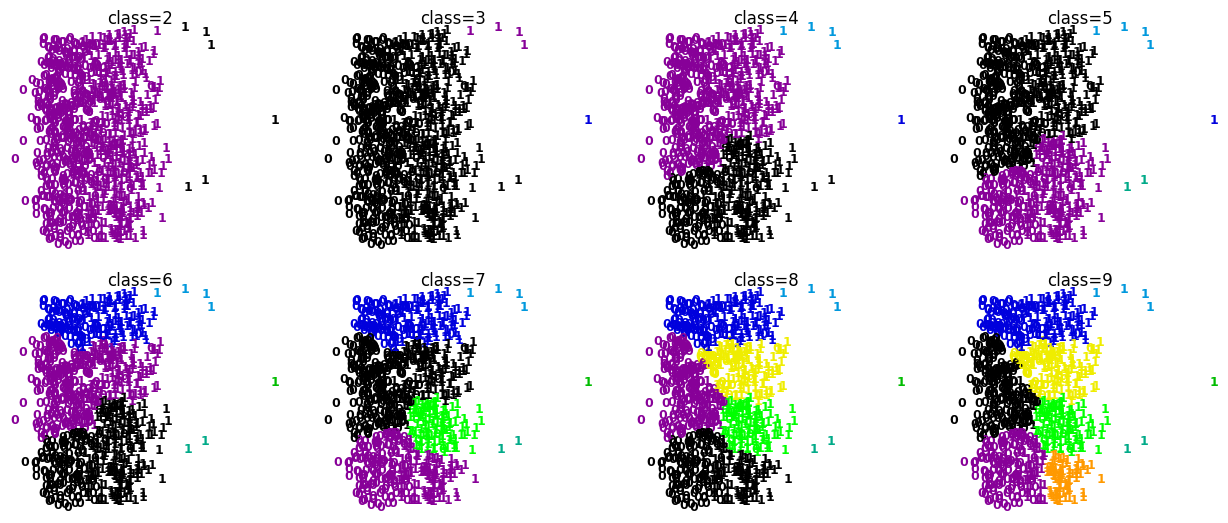
\includegraphics[width=15cm]{resource/pca_dec.png}
\caption{{\ttfamily PCA} 降维后均值距离层次聚类结果}
\label{fig:pca_dec}
\end{figure}

\section{分析与体会}
\begin{enumerate}
\item 本次实验中对各种聚类方法进行了系统性的实验,并且分析了各种方法的运行效果。我对聚类方法有了更加全面而深刻的认识;
\item 对于层次分类,课本上所学的三种距离度量都存在类别不均衡的问题,对偏差很大的样本缺乏抗性,而使用{\ttfamily Ward} 度量的方法可以很好解决这个问题;
\item {\ttfamily PCA} 降维有很大局限。在实验使用的数据集中{\ttfamily PCA} 降维会产生一些偏离的样本,效果不如一些非线性降维方法好。
\end{enumerate}

\section{程序代码及说明}
程序使用{\ttfamily Python} 编写,使用{\ttfamily scikit learn}。源代码参见 \url{https://github.com/chaonan99/university_homework/blob/pattern_recognition/h4/src/h4.ipynb}

\end{document}
